\documentclass[11pt]{article}
\usepackage[a4paper,margin=0.85in]{geometry}
\usepackage{amsmath,amssymb,amsthm,booktabs,array,graphicx,caption,subcaption}
\usepackage{url,natbib,microtype}
\usepackage[colorlinks=true,allcolors=blue]{hyperref}
\newtheorem{theorem}{Theorem}
\newtheorem{proposition}{Proposition}
\setlength{\parskip}{0.12em}
\setlength{\parindent}{1em}
\graphicspath{{../reports/selection_revision/figures/}{../reports/selection/figures/}}
% AUTOGENERATED; source manifest in reports/selection.
\newcommand{\SelectionUnits}{20}
\newcommand{\CandidateFits}{280}
\newcommand{\BestMetric}{Covariance TAR}
\newcommand{\BestRegret}{0.34}
\newcommand{\MeanTarRegret}{0.79}
\newcommand{\CheapProbeRegret}{0.47}
\newcommand{\CovarianceRegret}{0.34}
\newcommand{\CrossfitRegret}{0.47}
\newcommand{\LogmeRegret}{1.01}
\newcommand{\PrimaryRuntime}{723.2}
\newcommand{\ControlsRuntime}{308.3}
\newcommand{\UndefinedCrossfit}{0}

% AUTOGENERATED exploratory values.
\newcommand{\BestFixedRegret}{0.18}
\newcommand{\ProfileLogmeRegret}{0.92}
\newcommand{\AdaptiveHscoreRegret}{1.50}
\newcommand{\LodoRegret}{0.66}
\newcommand{\LogmeNonconverged}{10612}

% AUTOGENERATED follow-up values.
\newcommand{\ExpandedBestMetric}{covariance retention}
\newcommand{\ExpandedBestRegret}{0.395}
\newcommand{\ExpandedBoundaryCount}{2}
\newcommand{\ExpandedPlateauCount}{37}
\newcommand{\ExpandedFixedRegret}{0.425}

% Generated from verified revision artifacts.
\newcommand{\RevCovRegret}{0.221}
\newcommand{\RevLogmeRegret}{0.983}
\newcommand{\RevTunedRegret}{0.502}
\newcommand{\RevFixedRegret}{0.294}
\newcommand{\RevCovLogmeGain}{+0.762}
\newcommand{\RevCovLogmeCI}{$[+0.406, +1.196]$}
\newcommand{\RevCovFixedGain}{+0.073}
\newcommand{\RevCovFixedCI}{$[-0.056, +0.203]$}
\newcommand{\RevSvhnCovGain}{+0.316}
\newcommand{\RevSvhnCovCI}{$[+0.017, +0.639]$}
\newcommand{\RevSvhnLogmeGain}{-0.623}
\newcommand{\RevSvhnLogmeCI}{$[-1.004, -0.289]$}
\newcommand{\RevUpperGridCount}{5}
\newcommand{\RevHardware}{12th Gen Intel(R) Core(TM) i5-12450H}
\newcommand{\RevCrossfitUndefined}{6}
\newcommand{\RevLowerGridCount}{0}
\newcommand{\RevUpperImprovementCount}{0}
\newcommand{\RevHscoreRho}{-0.190}
\newcommand{\RevAdaptiveRho}{0.231}
\newcommand{\RevHeadSeconds}{0.072}
\newcommand{\RevHistoricalMaxDelta}{0.0481}
\newcommand{\RevHistoricalCovDelta}{+0.0000038}
\newcommand{\RevSvhnMajority}{19.59}

\title{Selecting Frozen Linear Patch Operators:\\An Empirical Audit under Matched Feature Budgets}
\author{Ankit Guin}
\date{November 2026}
\hypersetup{pdftitle={Selecting Frozen Linear Patch Operators: An Empirical Audit under Matched Feature Budgets},pdfauthor={Ankit Guin},pdfsubject={Controlled empirical audit of frozen linear patch representation selection}}
\begin{document}
\maketitle
\begin{abstract}
Can inexpensive statistical scores select compressed visual representations usefully when feature dimension, patch size and downstream regularization are controlled? We audit frozen shared linear patch operators with eleven selection rules on CIFAR-10, CIFAR-100 and an independent SVHN domain: two feature budgets, fourteen candidates and five training-subset seeds give 420 candidate heads in thirty evaluation units. Exact-content deduplication precedes training; selectors and validation-selected ridge penalties are frozen before evaluation on every official test image. Baselines include numerically refined profile-evidence LogME, adaptive H-score and diagnostic probes. A fixed DCT policy is developed on historical CIFAR evidence and locked before SVHN evaluation. Mean regrets are \RevCovRegret{} percentage points for covariance retention, \RevLogmeRegret{} for profile LogME and \RevFixedRegret{} for fixed DCT. However, covariance's pooled accuracy gain over fixed DCT is only \RevCovFixedGain{} points, with a paired 95\% seed/image interval of \RevCovFixedCI{}. Its SVHN choices also match an unlabeled reconstruction rule, and absolute SVHN accuracy is weak. Domain-specific outcomes, matched-patch-size comparisons, selection frequencies and measured time/memory therefore qualify aggregate rankings. The contribution is a controlled empirical decision audit with explicit development and evaluation boundaries; these observations do not establish that label-dependent selection is generally necessary or that one score is universally superior.
\end{abstract}

\section{Introduction}
Choosing a representation before fitting every downstream classifier can save time, but the selection step has its own label and computational costs. A representation that retains image variance or class-mean energy need not be the best input to a finite-sample regularized head. Consequently, small differences among statistical selectors are meaningful only relative to competitive implementations, uncertainty and a credible fixed-policy alternative.

Vision Transformers provide a concrete setting: ordered extraction of complete patches is reversible, whereas a subsequent linear map can reduce dimension~\citep{dosovitskiy2021vit}. Patch-size scaling and pixel-token studies already investigate trained architectures at much larger scale~\citep{wang2025scaling,nguyen2025pixels}. We ask a narrower question: \emph{can inexpensive statistical scores reliably select frozen compressed linear patch representations under matched feature budgets, and does the resulting accuracy gain justify selection cost?} We do not transfer a full pretrained encoder or infer end-to-end Transformer performance.

Our empirical contribution has three parts. First, a fourteen-candidate bank controls global rank and output dimension, with secondary comparisons also matching patch size and dense projection dimensions. Second, one unified revision cohort evaluates competitive evidence, shrinkage and probe baselines on content-clean training splits and full official test sets, including an external digit domain. Third, a CIFAR-developed fixed rule, paired image/seed uncertainty and fresh-process resource measurements test the practical value of task-aware selection. These experiments extend an earlier two-CIFAR preliminary study; they do not turn its exploratory findings into independent confirmations. The rank and Gaussian arguments supply established theoretical context, with proofs and synthetic controls in the appendix.

\section{Related work and precise scope}
H-score evaluates representations through class-conditional means and feature covariance~\citep{bao2019hscore}. LogME evaluates Bayesian linear-model evidence~\citep{you2021logme}. The published ECML PKDD study of \citet{ibrahim2023transferability} already identifies covariance-estimation problems, develops shrinkage H-score and evaluates substantially larger experiment collections. Covariance awareness and estimator instability are therefore prior art. Ledoit--Wolf shrinkage~\citep{ledoit2004covariance} and cross-validated contrast distances~\citep{diedrichsen2016crossvalidated} likewise precede this work.

Evaluation design is itself established research. \citet{agostinelli2022stable} show that transferability-metric orderings change with candidate pools, targets and evaluation measures. More recently, \citet{singh2026benchmark} show how static model hierarchies can favor dataset-agnostic heuristics. Our fixed-policy comparison directly addresses that concern within a deliberately restricted shared-patch bank; neither design sensitivity nor the usefulness of simple heuristics is claimed as a new general discovery. Unlike these broader source-model benchmarks, we vary raw-pixel patch operators under explicit scalar-output and projection-dimension constraints.

LEEP~\citep{nguyen2020leep} and negative conditional entropy~\citep{tran2019transferability} evaluate source predictions or labels. Random, PCA and DCT patch maps have no pretrained source classifier or source-label vocabulary. Attaching such a classifier would change this experiment and introduce source supervision; these methods are discussed but not assigned artificial source outputs. Our transferred DeiT condition uses only its patch matrix~\citep{touvron2021deit}, with its ImageNet-data advantage explicitly retained. Overlapping/convolutional stems and anti-aliasing are established architectural choices~\citep{wu2021cvt,xiao2021convs,qian2021alias}, outside the controlled bank. The study also differs from information-loss audits at multimodal connectors~\citep{li2025lost}. No exhaustive novelty or state-of-the-art claim is made.

\section{Scores and theoretical context}
For $x\in\mathbb R^{HWC}$, patch dimension $m=Cp^2$, token count $N=HW/p^2$ and $W\in\mathbb R^{d\times m}$, the complete ordered representation is $z=Ax+b$ with $A=(I_N\otimes W)Q_p$. Since $Q_p$ is a permutation, $\operatorname{rank}(A)=N\operatorname{rank}(W)$. Compression can discard directions without discarding every task's relevant signal. Appendix~\ref{sec:theory} records the elementary injectivity and collision arguments.

For balanced Gaussian classes $X\mid Y=y\sim\mathcal N(\mu+yv/2,\Sigma)$, $\Sigma\succ0$, standard equal-covariance discrimination gives
\begin{equation}\label{eq:general_gaussian}
R^*(AX)=\Phi\!\left(-\tfrac12\sqrt{v^\top A^\top(A\Sigma A^\top)^\dagger Av}\right).
\end{equation}
Only for isotropic covariance does this depend solely on Euclidean row-space alignment. This is established Gaussian theory, not a general natural-image accuracy formula.

At patch position $j$, let $B_j=\sum_c\pi_c(\mu_{cj}-\mu_j)(\mu_{cj}-\mu_j)^\top$, and let $P_W$ project onto the rows of $W$. Mean retention is
\begin{equation}\label{eq:mean_retention}
T_{\rm mean}=\frac{\sum_j\operatorname{tr}(P_WB_j)}{\sum_j\operatorname{tr}(B_j)}.
\end{equation}
It is an energy ratio, not mutual information. Equal population means make it undefined, even if nonlinear labels are recoverable; estimated means also contain sampling noise. Covariance retention replaces Euclidean energies by within-class-whitened energies:
\begin{equation}\label{eq:covret}
T_{\rm cov}=\frac{\sum_j\operatorname{tr}\{(WS_\lambda W^\top)^{-1}WB_jW^\top\}}
{\sum_j\operatorname{tr}(S_\lambda^{-1}B_j)},\quad
S_\lambda=(1-\lambda)S+\lambda\operatorname{tr}(S)I/m.
\end{equation}
Here $S$ pools within-class patch residual covariance across positions. This approximation omits cross-patch dependence and supplies no multiclass Bayes guarantee. The locked default is $\lambda=.1$; predetermined .01 and .5 values form a sensitivity analysis. Cross-fitted retention replaces squared contrasts by cross-inner-products between independent stratified diagnostic halves. Its components can be unbiased for a fixed independent operator, but the ratio need not be; nonpositive denominators trigger a disclosed uniform fallback.

Rank, reconstruction retention, fixed-shrinkage H-score, adaptive H-score, profile LogME and diagnostic probes complete the comparison. Adaptive H-score uses Ledoit--Wolf covariance and the $(1-\alpha)$ correction~\citep{ibrahim2023transferability}. Profile LogME uses the published integrated Gaussian evidence objective, profiles the noise precision analytically, searches a broad log prior/noise-ratio grid, refines interior maxima and compares the analytic infinite-ratio null limit. All classwise refinement statuses and bounds are saved; failed refinement aborts the unit. Features are centered and divided by a single RMS scalar; one-hot targets are uncentered. This is an independent, numerically checked implementation, not a claim of bitwise reproduction of author code. The eleven-step implementation is retained only in the preliminary results.

\section{Revision experimental protocol}
\paragraph{Domains and label budgets.}
We use official CIFAR-10/100~\citep{krizhevsky2009cifar} and cropped SVHN~\citep{netzer2011svhn} train/test partitions at native $32\times32$ RGB resolution, fixed ImageNet channel normalization and no augmentation. Seeds 10--14 each draw 1,000 operator-fit, 1,000 diagnostic and 500 validation images, balanced within each training subset. Operators fit without labels; downstream heads use labels from both operator and diagnostic subsets, totaling 2,000 training labels. Selectors use the same 1,000 diagnostic labels; validation consumes another 500 labels. Fixed DCT uses no diagnostic labels for selection, although the common head-training protocol remains unchanged. These budgets refer to distinct roles, not an additional 1,000 head-training images.

\paragraph{Content separation and full testing.}
Before sampling, SHA256 hashes of raw pixels identify exact duplicates. Training rows matching any official test content, all conflicting-label training-content groups, and repetitions after the first otherwise valid training occurrence are removed. This uses test images, never test labels. Operator, diagnostic and validation content sets are pairwise disjoint and test-disjoint. All official test images remain: 10,000 for each CIFAR dataset and 26,032 for SVHN, with natural test class frequencies. Repeated test content is disclosed and retained to preserve the full official benchmark. Near duplicates are not certified absent. CIFAR-100 loses 10 training rows matching test content, 18 rows in conflicting-label groups and five additional repeated rows. Exact IDs, exclusion counts, hashes and class counts accompany the evidence.

\paragraph{Operators and matched budgets.}
For $p\in\{2,4,8,16\}$ and budget $B\in\{256,768\}$, set $d=B/N$. Each patch size has random orthonormal, low-frequency DCT and unlabeled PCA maps; PCA uses at most 8,000 operator-fit patches. DCT includes a fixed orthonormal color transform. At $p=16$, add SVD-truncated DeiT-tiny patch weights and their orthonormal-row counterpart, giving fourteen candidates. The pair spans the same retained subspace with different singular scaling. Each candidate has global rank $B$ and equal linear-head parameter count within a budget. Dense projection cost is $2B(3p^2)$ multiply/add FLOPs per image; equal feature count does not equal equal tokenization or Transformer compute. Within-$p,B$ comparisons separately match projection dimensions. Only the patch matrix is transferred, with external ImageNet data and an original-resolution mismatch disclosed.

\paragraph{Heads, probes and frozen choices.}
Multiclass least-squares ridge heads are solved by eigendecomposition. A thirteen-value grid, $\{10^{-2},10^{-1},\ldots,10^{10}\}$, selects penalties by validation accuracy; ties favor larger penalties. The common scalar normalization preserves orthogonal-coordinate invariance. The fixed diagnostic probe fits 500 diagnostic images and evaluates the other 500 with penalty 10. Its tuned counterpart maximizes diagnostic held-out accuracy over the same thirteen-value grid; that joint candidate/penalty search can overfit its small diagnostic evaluation half and is not treated as an unbiased accuracy estimate. No official test labels choose candidates or penalties. All scores, eligible tie sets, sensitivity choices, head penalties and within-p choices are serialized before any test predictions, then verified unchanged by hash.

\paragraph{Fixed policy and development boundary.}
The policy $p04\_dct$ is locked at both budgets using already observed historical CIFAR evidence. Its SVHN result is prospective evaluation on an independent domain. Its revised CIFAR performance remains descriptive because those domains informed policy development. Fresh CIFAR seeds improve repeatability, not domain independence. The local revision protocol and one documented pre-final-run penalty-grid amendment are distributed with the code; this is not an external preregistration. A partial narrower-grid revision run is preserved and excluded. The original preliminary and exploratory CIFAR cohorts remain available separately.

\paragraph{Endpoints and uncertainty.}
Selection accuracy is the uniform expectation across maximizing candidates; undefined scores fall back to uniform bank choice and are counted. Regret is best observed candidate test accuracy minus selected accuracy, relative to a noisy finite-bank empirical oracle. Spearman correlation measures within-bank ranking; constant scores have undefined correlation. We report each domain and budget, selection frequencies and absolute accuracies alongside regret.

Paired intervals resample training-seed blocks within each observed domain, preserving budgets and selectors. A joint bootstrap also resamples common test-image weights shared across every seed, budget and selector in that domain. A multinomial over joint correctness patterns implements exactly the image bootstrap for paired mean accuracy, without treating repeated test images across seeds as independent replications. Domains receive equal aggregate weight; the domains themselves are not resampled as a credible population sample. We retain 4,000 draws, seed-only and joint intervals, and all reference comparisons. These intervals are conditional on the observed domains and models. They omit policy-development uncertainty, broader domain variation, near-duplicate dependence and multiple-comparison correction. They support neither a universal winner nor an equivalence claim from an interval containing zero.

\section{Results}
\subsection{Per-domain performance and competitive baselines}
\begin{table}[tb]\centering\small
\caption{Revision selection regret (percentage points), averaged over seeds and budgets. The three observed domains receive equal weight. Rank uses uniform tie expectations; correlations are within candidate banks, then averaged. A fixed policy supplies no meaningful full-bank ranking, so its correlation is omitted.}\label{tab:revision}
\begin{tabular}{lrrrrr}\toprule
Selector & CIFAR-10 & CIFAR-100 & SVHN & Mean & $\rho$\\\midrule
Rank / uniform ties & 3.106 & 1.454 & 0.627 & 1.729 & --\\
Reconstruction & 0.772 & 0.356 & 0.240 & 0.456 & 0.489\\
Mean retention & 0.772 & 0.356 & 0.240 & 0.456 & 0.528\\
Covariance retention & 0.249 & 0.174 & 0.240 & 0.221 & 0.473\\
Cross-fitted retention & 0.643 & 0.162 & 0.514 & 0.440 & 0.554\\
Fixed H-score & 5.330 & 4.002 & 2.008 & 3.780 & -0.190\\
Adaptive H-score & 0.992 & 1.607 & 0.197 & 0.932 & 0.231\\
Profile LogME & 0.452 & 1.318 & 1.180 & 0.983 & 0.337\\
Diagnostic probe & 0.302 & 0.214 & 0.491 & 0.336 & 0.410\\
Tuned diagnostic probe & 0.571 & 0.414 & 0.522 & 0.502 & 0.418\\
Fixed DCT (p=4) & 0.253 & 0.072 & 0.556 & 0.294 & --\\
\bottomrule\end{tabular}
\end{table}

\begin{table}[tb]\centering\small
\caption{Full-test absolute accuracy (percent). Oracle selects by test outcomes only as a descriptive upper reference. Cov., LogME, Probe and DCT denote covariance retention, profile LogME, tuned diagnostic probe and locked fixed DCT.}\label{tab:absolute}
\begin{tabular}{lrrrrrr}\toprule
Domain & $B$ & Oracle & Cov. & LogME & Probe & DCT\\\midrule
CIFAR-10 & 256 & 36.00 & 35.87 & 35.43 & 35.28 & 35.87\\
CIFAR-10 & 768 & 35.49 & 35.12 & 35.15 & 35.07 & 35.11\\
CIFAR-100 & 256 & 10.85 & 10.85 & 8.98 & 10.60 & 10.85\\
CIFAR-100 & 768 & 10.73 & 10.39 & 9.97 & 10.16 & 10.60\\
SVHN & 256 & 16.68 & 16.40 & 14.79 & 16.33 & 15.87\\
SVHN & 768 & 16.89 & 16.70 & 16.43 & 16.20 & 16.59\\
\bottomrule\end{tabular}
\end{table}

Tables~\ref{tab:revision} and \ref{tab:absolute} separate selection regret from absolute low-label classification accuracy. Mean regrets are \RevCovRegret{} points for covariance retention, \RevLogmeRegret{} for profile LogME, \RevTunedRegret{} for the tuned diagnostic probe and \RevFixedRegret{} for fixed DCT. These thirty units contain three domains, not thirty independent classification problems. The CIFAR development and external-domain roles must remain distinct even when averaging their observations.

Mean retention and unlabeled reconstruction select the same $p16\_pca$ candidate in all thirty units. On SVHN, covariance retention also chooses that candidate in all ten units. Its external-domain gain over fixed DCT therefore does not demonstrate a benefit of label-dependent scoring: an unlabeled rule attains the same selections there. Adaptive H-score has the lowest observed SVHN regret, while fixed DCT has the lowest CIFAR-100 regret; the pooled ordering is not a universal one. Cross-fitted retention is undefined in \RevCrossfitUndefined{} of thirty units and uses the declared uniform fallback; these failures are included in its reported regret.

The independent-domain task is also weak for this bank/head combination: its mean bank-oracle accuracies are below the SVHN test majority-class frequency of \RevSvhnMajority{}\%. This test-informed constant-class reference is descriptive, not a new prospective selector. Table~\ref{tab:balance} adds explicitly secondary balanced-accuracy context because training subsets are balanced whereas SVHN's test distribution is not. It does not replace the locked ordinary-accuracy endpoint. Small regret and a positive conditional selection gain do not establish a useful or competitive SVHN classifier.

\begin{figure}[tb]\centering
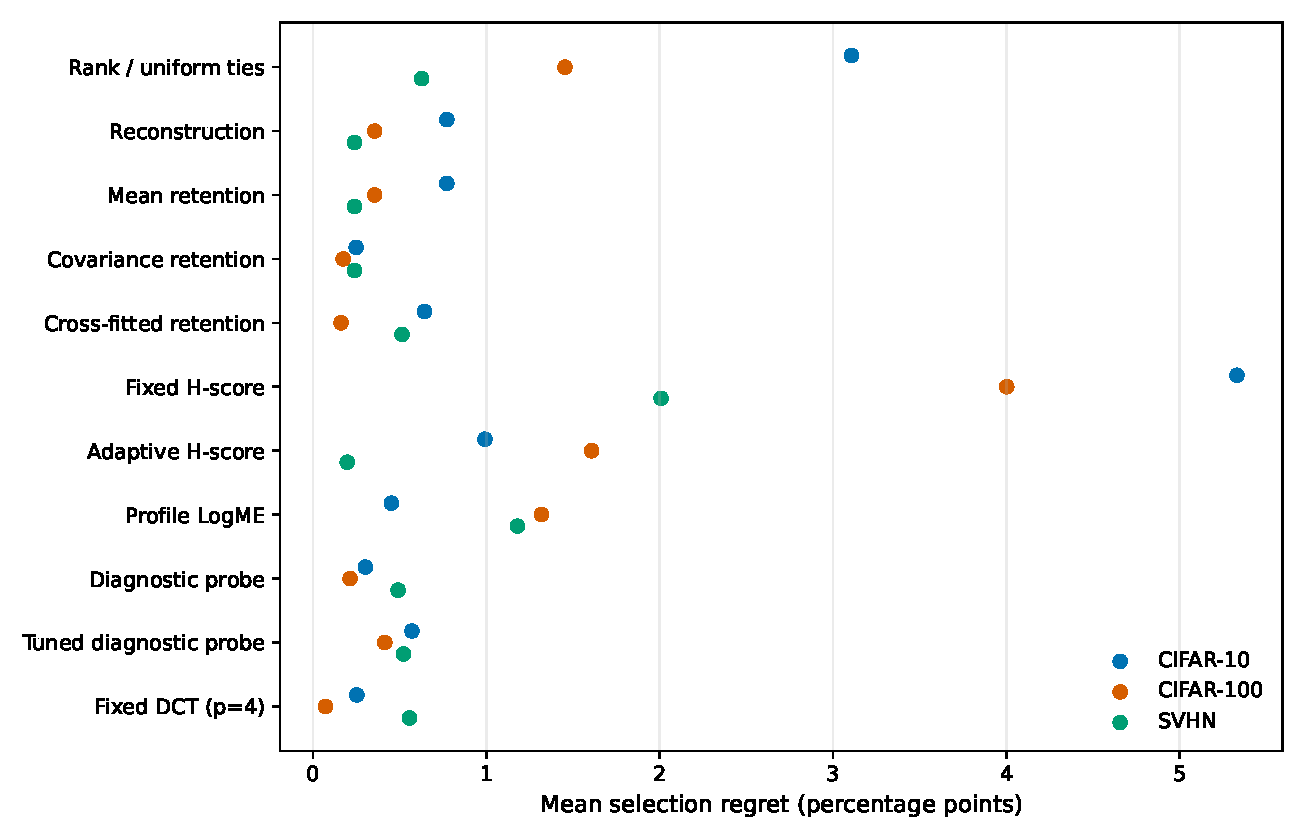
\includegraphics[width=.94\linewidth]{regret_by_domain.pdf}
\caption{Revision mean regret by observed domain, averaged over seeds and budgets. Domain-dependent orderings are visible without treating repeated seeds as new domains. Paired intervals are reported separately.}\label{fig:domains}
\end{figure}

\subsection{Does task-aware selection improve on fixed DCT?}
\begin{table}[tb]\centering\small
\caption{Paired accuracy gain over fixed DCT, in percentage points, with 95\% joint seed/image bootstrap intervals. Only SVHN provides independent prospective evaluation of the CIFAR-developed fixed policy. The pooled column is descriptive. Full seed-only and all pairwise-reference results accompany the code.}\label{tab:paired}
\begin{tabular}{lrr}\toprule
Selector & Three-domain gain [CI] & SVHN gain [CI]\\\midrule
Covariance retention & +0.073 [-0.056, +0.203] & +0.316 [+0.017, +0.639]\\
Profile LogME & -0.689 [-1.104, -0.355] & -0.623 [-1.004, -0.289]\\
Adaptive H-score & -0.638 [-1.133, -0.180] & +0.359 [+0.036, +0.689]\\
Diagnostic probe & -0.042 [-0.155, +0.072] & +0.065 [-0.136, +0.268]\\
Tuned diagnostic probe & -0.209 [-0.426, -0.002] & +0.034 [-0.441, +0.456]\\
\bottomrule\end{tabular}
\end{table}

The overall covariance-minus-profile-LogME accuracy difference is \RevCovLogmeGain{} percentage points, with joint 95\% interval \RevCovLogmeCI{}. A small point difference alone does not establish useful superiority. The independent SVHN covariance-minus-fixed-policy gain is \RevSvhnCovGain{} points, interval \RevSvhnCovCI{}; the corresponding profile-LogME gain is \RevSvhnLogmeGain{}, interval \RevSvhnLogmeCI{}. Table~\ref{tab:paired} makes the fixed-policy comparison explicit rather than treating an expensive selector's proximity to the bank oracle as sufficient practical evidence. Equal scores or overlapping intervals do not prove equivalence.

\subsection{Candidate choices, matching and numerical sensitivity}
\begin{table}[tb]\centering\small
\caption{Most frequently selected candidate, with fractional counts for tied selections. All candidate frequencies, including remaining mass, are supplied as CSV. SVHN contains ten dataset/seed/budget units, not ten independent domains.}\label{tab:frequencies}
\begin{tabular}{llrlr}\toprule
Selector & Modal candidate & Count & SVHN modal candidate & Count\\\midrule
Mean retention & p16\_pca & 30/30 & p16\_pca & 10/10\\
Covariance retention & p04\_dct & 10/30 & p16\_pca & 10/10\\
Profile LogME & p16\_deit\_native\_svd & 7/30 & p16\_deit\_native\_svd & 4/10\\
Adaptive H-score & p16\_pca & 21/30 & p16\_pca & 7/10\\
Tuned diagnostic probe & p16\_random & 6/30 & p16\_random & 3/10\\
Fixed DCT (p=4) & p04\_dct & 30/30 & p04\_dct & 10/10\\
\bottomrule\end{tabular}
\end{table}

\begin{table}[tb]\centering\small
\caption{Regret within matched patch size and feature budget, in percentage points, averaged over the three domains and five seeds. The fixed p=4 policy has no within-p analogue at other patch sizes and is omitted.}\label{tab:matched}
\begin{tabular}{lrrrr}\toprule
Patch size & Covariance & LogME & Adaptive H & Tuned probe\\\midrule
2 & 0.211 & 0.470 & 0.760 & 0.412\\
4 & 0.124 & 0.339 & 0.781 & 0.281\\
8 & 0.109 & 0.153 & 0.423 & 0.263\\
16 & 0.273 & 0.600 & 0.378 & 0.545\\
\bottomrule\end{tabular}
\end{table}

\begin{table}[tb]\centering\small
\caption{Predetermined covariance-shrinkage sensitivity: mean regret in percentage points. Lambda=0.1 is the locked default; no setting is chosen retrospectively for the main comparison.}\label{tab:shrinkage}
\begin{tabular}{lrrrr}\toprule
$\lambda$ & CIFAR-10 & CIFAR-100 & SVHN & Mean\\\midrule
0.01 & 0.249 & 0.078 & 0.240 & 0.189\\
0.1 & 0.249 & 0.174 & 0.240 & 0.221\\
0.5 & 0.239 & 0.202 & 0.240 & 0.227\\
\bottomrule\end{tabular}
\end{table}

Table~\ref{tab:frequencies} reports modal selections; complete fractional counts expose remaining candidate mass. Table~\ref{tab:matched} restricts each comparison to one patch size and budget, hence matching dense projection dimensions. Each smaller bank has its own test oracle, so its regret cannot be compared directly with full-bank regret as if the decision problem were unchanged. Table~\ref{tab:shrinkage} keeps every predetermined covariance setting; it does not select a favorable shrinkage value after testing.

The lower and upper grid endpoints were selected by \RevLowerGridCount{} and \RevUpperGridCount{} of 420 heads, respectively; \RevUpperImprovementCount{} paths strictly improve from the penultimate to the largest penalty. Accuracy ties favor larger penalties, so an endpoint can indicate a plateau rather than monotonic improvement; complete validation paths are retained. The finite grid does not certify a continuous optimum. Classwise profile-evidence convergence records replace the short iteration cap as the main baseline.

Fixed H-score's mean within-bank rank correlation is \RevHscoreRho{}, versus \RevAdaptiveRho{} for adaptive H-score. The released family-by-domain audit records both scores, adaptive shrinkage and actual head accuracy. This distinguishes an implementation/convergence check from an empirical ranking failure: all fixed-shrinkage covariance systems are positive definite, adaptive shrinkage is estimated from the same diagnostic data, and native/orthonormal DeiT maps separately expose conditioning sensitivity. These controls do not identify a single causal explanation for poor H-score behavior; cross-patch dependence, regularization and a restricted operator family remain plausible sources of mismatch. No favorable transformation is selected using test accuracy.

\subsection{Computational value}
\begin{table}[tb]\centering\small
\caption{Selection costs on identical CPU hardware (two numerical threads): median of three fresh-process repeats for each domain and budget, at seed 10. Warm time includes all required extraction, statistics and scoring; cold includes bank fitting once. Peak RSS includes cold operator construction; incremental RSS is relative to the loaded-input baseline (10 ms sampling). Input decoding, imports, downstream head fitting and test inference are excluded. Regret repeats the full-cohort mean from Table~\ref{tab:revision}.}\label{tab:cost}
\begin{tabular}{lrrrrr}\toprule
Selector & Warm (s) & Cold (s) & RSS (MiB) & $\Delta$RSS & Regret\\\midrule
Rank / uniform ties & 0.043 & 0.313 & 433 & 148 & 1.729\\
Reconstruction & 0.566 & 0.826 & 518 & 234 & 0.456\\
Mean retention & 0.574 & 0.829 & 518 & 234 & 0.456\\
Covariance retention & 0.872 & 1.161 & 517 & 233 & 0.221\\
Cross-fitted retention & 0.572 & 0.829 & 518 & 234 & 0.440\\
Fixed H-score & 1.623 & 2.090 & 497 & 212 & 3.780\\
Adaptive H-score & 1.799 & 2.126 & 503 & 218 & 0.932\\
Profile LogME & 3.034 & 3.282 & 500 & 214 & 0.983\\
Diagnostic probe & 1.932 & 2.271 & 497 & 211 & 0.336\\
Tuned diagnostic probe & 1.926 & 2.262 & 497 & 211 & 0.502\\
Fixed DCT (p=4) & $<0.001$ & $<0.001$ & 285 & $<1$ & 0.294\\
\bottomrule\end{tabular}
\end{table}

Resource measurements include the feature extraction and statistics needed to score all candidates. Each method runs in a fresh process on identical hardware, at two numerical-library threads, for seed 10 of every domain/budget, repeated three times. Bank fitting is shared for task-aware methods; fixed DCT constructs only its specified operator and requires no bank search. Warm selection assumes candidate operators are already fitted; cold selection includes their actual fitting cost once. Downstream selected-head fitting and test inference are excluded and separately recorded. Median head fitting per candidate is \RevHeadSeconds{} seconds in the final cohort. Such inexpensive heads mean that avoiding a full-bank fit does not automatically yield a net application speedup; selector overhead can be a material part of the low-label computation.

Peak resident memory includes the Python/scientific runtime and loaded operators, so incremental sampled RSS is also provided. Ten-millisecond sampling can miss brief peaks. The reference implementation uses a comprehensive shared patch-statistics routine; when benchmarking a patch-retention method alone, its full routine cost is charged, including reusable components. Specialized minimal implementations could be faster. The measured cost/accuracy tradeoff, rather than a universal asymptotic speedup, is the practical result. A fixed-policy accuracy close to that of task-aware selection remains a reason to use the fixed policy unless a particular application values the measured gain enough to pay for selection.

In this implementation, covariance retention is faster than profile LogME and either diagnostic probe, with slightly higher peak memory. Fixed DCT has negligible selection cost. Thus covariance retention offers a measured time advantage over other label-dependent comparators, while its uncertain pooled accuracy gain over the fixed rule and the low cost of head fitting limit a broader efficiency argument.

\section{Discussion and limitations}
The central contribution is a controlled empirical decision audit. Existing transferability work already establishes covariance-estimation instability, candidate-pool dependence and the possibility of strong fixed heuristics. Our narrower evidence examines those issues for shared frozen linear raw-pixel patch maps while fixing output dimension and separately matching projection dimensions. It explicitly evaluates what additional diagnostic labels and computation buy over a developed fixed rule.

Within this final bank, covariance retention has the lowest pooled observed regret and a positive conditional accuracy difference from profile LogME. Its pooled gain over fixed DCT remains small with uncertainty spanning zero, and its SVHN selections are identical to unlabeled reconstruction. Thus the evidence supports a conditional comparison of scoring rules, while failing to establish that label-dependent selection is generally necessary. Weak absolute SVHN accuracy further limits any claim of practical downstream utility. These negative conclusions are central results of the audit.

Three domains improve on a two-CIFAR study but still support limited external generalization: SVHN is one independent digit domain, not a diverse collection of application domains. There is no medical, satellite, segmentation or full-encoder experiment. Five training-subset seeds quantify within-domain repeatability. CIFAR-10 and CIFAR-100 remain related datasets; neither is independent policy validation. SVHN uses its official naturally imbalanced test distribution, while training subsets are class balanced. Cross-domain aggregate accuracies should not be mistaken for comparable task difficulty.

The diagnostic bank is restricted to fourteen candidates, two dimensions and linear heads trained on only 2,000 labels. A metric's failure to predict this regularized finite-sample head does not disprove representation sufficiency or imply failure under end-to-end adaptation. The ImageNet-transferred patch condition has external supervision and scale mismatch; no full DeiT accuracy claim follows. Matching patch size and output dimension controls dense projection geometry, not entire-model compute. The covariance-retention approximation ignores cross-patch dependence, and its shrinkage settings cover only a small predetermined range.

Regret uses the maximum of noisy observed test accuracies and is descriptive. Paired accuracy differences avoid claiming an unbiased population oracle, but the conditional bootstrap does not cover unseen domains or every source of dependence. Exact-content filtering removes detected leakage before final training, yet cannot certify absence of near duplicates. The fixed policy was selected with historical CIFAR results, and even its independent SVHN evaluation is one held-out domain. The public release is versioned and checksum-verifiable; no archival DOI or completed independent installation on another platform is claimed.

\section{Reproducibility and conclusion}
The revision distribution contains versioned source, a locked environment specification, the local protocol/configuration, official indices and content audits, operator matrices, selected heads, validation paths, pretest choices, full predictions, checksum manifests, replay tools and table/figure generation scripts. Code, the manuscript and matching source/evidence archives are supplied in the \href{https://github.com/AnkitGuin/Task-Dependent-VIT-Patch-Loss/releases/tag/v2026.11.15-v2}{public repository release v2026.11.15-v2}. Per-file SHA256 manifests and external ZIP checksums identify the version; the tagged source and reproduction guide explain all cohorts. Raw dataset images and full pretrained-model files are excluded; preparation verifies their published checksums. Third-party attribution and the DeiT license accompany derived patch matrices. The preliminary study and exploratory follow-ups remain explicitly separate from the final cohort. The supplied reviewer-response document maps each criticism to changes and evidence. This is a public versioned release, not a claim of an issued archival DOI or independent scientific replication.

For these frozen linear patch banks, statistical selection must be judged against both a competitive evidence/probe baseline and a fixed rule developed outside the evaluation domain. Full-test, paired and cost measurements make that judgment reviewable without elevating small conditional differences into general superiority. The resulting benchmark is a scoped empirical contribution; broader claims require more independent domains and downstream model families.

\clearpage
\appendix
\section{Mathematical results}\label{sec:theory}
\paragraph{Conventions.} Let $X\in\mathbb R^{H\times W\times C}$ and let $x=\mathrm{vec}(X)\in\mathbb R^n$, $n=HWC$. Assume $p\mid H,W$ and the patch ordering is fixed and known. Put $m=p^2C$ and $N=HW/p^2$. Throughout, all algebraic statements use exact arithmetic unless otherwise stated.

\begin{theorem}[Lossless ordered raw extraction]\label{thm:reshape}
The map which extracts every $p\times p$ patch, retains every pixel and the patch order, and concatenates all entries, is a permutation $Q_p\in\mathbb R^{n\times n}$. Therefore $Q_p^{-1}=Q_p^\top$, $Q_p^\top Q_p=I_n$, and $\|Q_p x\|_2=\|x\|_2$ for all $x$.
\end{theorem}
\begin{proof}
Every input entry is assigned to exactly one patch and one patch coordinate because patches partition the image grid, and each such coordinate is assigned to exactly one input entry. Thus each row and each column in the extraction matrix contains exactly one unit entry; all other entries are zero. Such a permutation matrix has orthonormal rows and columns. Multiplying by its transpose reverses the permutation, and its squared norm is unchanged.
\end{proof}
The conclusion does not cover dropping border pixels, treating tokens as an unordered set, quantization, or applying a stride/filter that discards dimensions. In particular a patch size above one is \emph{not} itself a rank-reducing operation.

\begin{proposition}[Rank criterion]\label{prop:rank}
For a fixed shared per-patch linear map $W\in\mathbb R^{d\times m}$, with complete ordered token output and a known additive offset, define
\begin{equation}\label{eq:operator}
 A=(I_N\otimes W)Q_p\in\mathbb R^{Nd\times n}.
\end{equation}
Then $\mathrm{rank}(A)=N\mathrm{rank}(W)$ and $\dim\ker A=N(m-\mathrm{rank}(W))$. Moreover $A$ is injective if and only if $\mathrm{rank}(W)=m$.
\end{proposition}
\begin{proof}
Right multiplication by the invertible $Q_p$ leaves rank unchanged. The Kronecker factor is block diagonal with $N$ copies of $W$, so its row and column spaces decompose as a direct sum over patches, and its rank is exactly $N\mathrm{rank}(W)$. Rank--nullity and $n=Nm$ yield the nullity. Injectivity holds precisely when the nullity is zero, equivalently $\mathrm{rank}(W)=m$. A fixed affine offset disappears when comparing two token outputs.
\end{proof}
The proposition does not imply that every observed finite sample contains a collision. Full column rank requires $d\ge m$ but mere width $d\ge m$ is not enough unless the matrix genuinely has full column rank. It also does not guarantee numerical stability for ill-conditioned matrices.

\begin{proposition}[Constructed label collision]\label{prop:collision}
Fix a $W$ with $\mathrm{rank}(W)<m$. There exist distinct images $x_\pm\in[0,1]^n$ satisfying $Ax_+=Ax_-$, and a balanced binary task with full-image optimal 0--1 risk zero but token-only risk $1/2$.
\end{proposition}
\begin{proof}
Choose $u\in\ker W$, $\|u\|_2=1$, and patch index $j$. Let $\delta=Q_p^\top(e_j\otimes u)$, and choose an interior base image $b\in[0.34,0.66]^n$. For any $0<\epsilon\le 0.2/\|u\|_\infty$, define $x_\pm=b\pm\epsilon\delta$. They are distinct because $\delta\ne0$, and valid in $[0,1]^n$. By construction,
\begin{equation}\label{eq:collision}
 Ax_+-Ax_-=2\epsilon(I_N\otimes W)(e_j\otimes u)=0.
\end{equation}
Let $\Pr[(X,Y)=(x_+,1)]=\Pr[(X,Y)=(x_-,0)]=1/2$. Seeing $X$ identifies $Y$ without error. But the same token value occurs for both labels and its posterior is $(1/2,1/2)$, so every token classifier has error $1/2$.
\end{proof}
This establishes only an \emph{adversarially chosen task for a fixed projection}; a learned $W$ can rotate away from the original null space. It does not show that real-world classes usually collide under ViT tokenization.

\begin{theorem}[Exact Gaussian Bayes risk]\label{thm:gaussian}
Let $Y\in\{-1,+1\}$ have equal prior probabilities and
\begin{equation}\label{eq:gauss_model}
 X\mid Y=y\sim\mathcal N(\mu+yv/2,\sigma^2I_n),\qquad\sigma>0.
\end{equation}
For any fixed deterministic linear representation $Z=AX+b$, define
\begin{equation}\label{eq:projector}
 P_A=A^\top(AA^\top)^\dagger A.
\end{equation}
Then, writing $\Phi$ for the standard normal CDF, its optimal 0--1 risk is
\begin{equation}\label{eq:bayes}
 \boxed{R^*(Z)=\Phi\left(-\frac{\|P_Av\|_2}{2\sigma}\right)}.
\end{equation}
For the raw image, $R^*(X)=\Phi(-\|v\|_2/(2\sigma))$.
\end{theorem}
\begin{proof}
Conditionally, $Z\mid Y=y\sim\mathcal N(A\mu+b+yAv/2,\sigma^2AA^\top)$. Both distributions are supported on the same affine subspace even when $A$ is rank-deficient. Equal priors and equal covariances imply the likelihood-ratio rule on that support: decide $+1$ when
\begin{equation}\label{eq:discriminant}
 S=(Av)^\top(\sigma^2 AA^\top)^\dagger(Z-A\mu-b)\ge0.
\end{equation}
Set $D^2=v^\top A^\top(AA^\top)^\dagger Av=v^\top P_A v=\|P_A v\|_2^2$. Then $S\mid Y=y$ is univariate normal with mean $yD^2/(2\sigma^2)$ and variance $D^2/\sigma^2$. If $D>0$, either conditional misclassification probability equals $\Phi(-D/(2\sigma))$. If $D=0$, the two feature distributions coincide and any constant prediction has error $1/2$, agreeing with $\Phi(0)$. Applying the same calculation with $A=I_n$ gives the raw-image expression.
\end{proof}
The formula is \emph{exact only} under the equal-prior, shared isotropic Gaussian model and fixed linear representation with complete observed output. It is not a general natural-image Bayes bound or a characterization of arbitrary nonlinear transformers. In particular it yields the three extremes
\begin{align}
 v\in\ker A&\implies R^*(Z)=1/2,\label{eq:nullcase}\\
 v\in\operatorname{row}(A)&\implies R^*(Z)=R^*(X),\label{eq:rowcase}\\
 \mathrm{rank}(A)=n&\implies R^*(Z)=R^*(X).\label{eq:fullcase}
\end{align}

\begin{proposition}[Data processing and task sufficiency]\label{prop:dpi}
For discrete $Y$ and any deterministic $Z=P(X)$, $I(Y;Z)\le I(Y;X)$ and $R^*(Z)\ge R^*(X)$. Both inequalities can be equalities even if $P$ is noninjective.
\end{proposition}
\begin{proof}
The first follows from the Markov chain $Y\to X\to Z$ by the data-processing inequality~\citep{coverthomas2006}. Every measurable decision rule based on $Z$ is also a measurable decision rule based on $X$ by composition, so its infimum risk cannot be smaller than the raw-image infimum. Equality holds whenever the conditional label distribution (or, for the 0--1 risk inequality, a Bayes-optimal decision) factors through $Z$.
\end{proof}
For a nonzero contrast vector define the task-alignment retention coefficient
\begin{equation}\label{eq:tar}
 \alpha(v;A)=\frac{\|P_Av\|_2}{\|v\|_2},\qquad \mathrm{TAR}=\alpha(v;A)^2.
\end{equation}
For shared patch maps, this projector acts separately with $P_W=W^\top(WW^\top)^\dagger W$ after the permutation $Q_p$; it is not necessary to form the massive matrix $A$. No theorem above guarantees that mean-based TAR predicts XOR, class covariance differences, optimization, translation invariance, or generalization after learned embedding updates.


\section{Secondary class-prior context}
\begin{table}[tb]\centering\small
\caption{Secondary, post-outcome class-prior context. Majority is the observed test majority-class frequency (a test-informed descriptive constant-class reference, not a prospectively selected rule). Remaining columns are macro-average class recall (balanced accuracy, percent); the oracle is defined on that secondary endpoint. Primary selection and regret remain ordinary full-test accuracy.}\label{tab:balance}
\begin{tabular}{lrrrrrr}\toprule
Domain & $B$ & Majority & Bal. oracle & Bal. cov. & Bal. LogME & Bal. DCT\\\midrule
CIFAR-10 & 256 & 10.00 & 36.00 & 35.87 & 35.43 & 35.87\\
CIFAR-10 & 768 & 10.00 & 35.49 & 35.12 & 35.15 & 35.11\\
CIFAR-100 & 256 & 1.00 & 10.85 & 10.85 & 8.98 & 10.85\\
CIFAR-100 & 768 & 1.00 & 10.73 & 10.39 & 9.97 & 10.60\\
SVHN & 256 & 19.59 & 16.64 & 16.30 & 14.73 & 15.95\\
SVHN & 768 & 19.59 & 16.74 & 16.65 & 16.41 & 16.54\\
\bottomrule\end{tabular}
\end{table}

Balanced accuracy is a post-outcome descriptive sensitivity endpoint. It is not used to reselect any main tokenizer or penalty, and no secondary bootstrap superiority claim is made. The empirical test-majority reference uses test labels and must not be reported as a prospectively developed classifier. Because CIFAR official test classes are balanced, its ordinary and balanced accuracies agree; SVHN's naturally imbalanced official test distribution motivates the additional context.

\section{Mean-retention null and distributional controls}
For one patch, sample two independent Gaussian classes from the same isotropic distribution with fixed positive sample counts. For a fixed rank-$r$ orthogonal projector in dimension $m$, $0<r<m$, the empirical squared-mean-difference retention has distribution $\operatorname{Beta}(r/2,(m-r)/2)$ and expectation $r/m$. In a projector-adapted basis, retained and discarded Gaussian squared norms are independent chi-squared variables; their variance factor cancels in the ratio. The population ratio remains undefined under equal class means. Increasing samples shrinks unnormalized noise energy, not its ratio into a valid information fraction.

The historical supporting control generated 4,000 independent null tasks per sample size and compared observed ratios to the analytic Beta law. A separate anisotropic Gaussian control uses two rank-one maps with equal Euclidean retention .5 but analytic risks approximately .00020 and .45549. Token-space Monte Carlo agrees within the recorded pointwise binomial intervals. These controls validate implementations under their stated distributions, not a universal natural-image theorem.
\begin{figure}[htb]\centering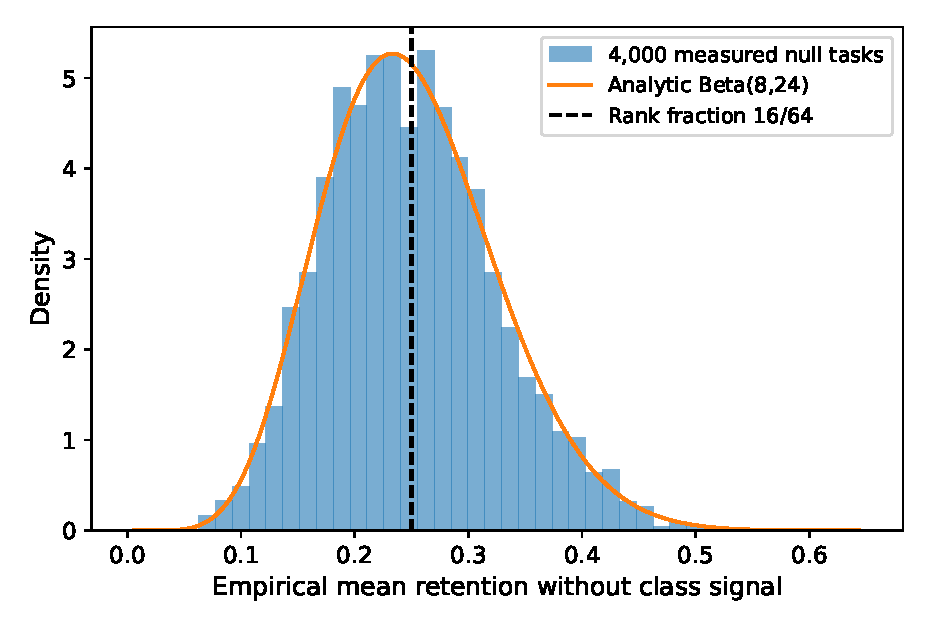
\includegraphics[width=.83\linewidth]{null_tar_calibration.pdf}
\caption{Supporting null calibration, enlarged for readability. Positive empirical mean retention occurs without population class separation.}\end{figure}
\begin{figure}[htb]\centering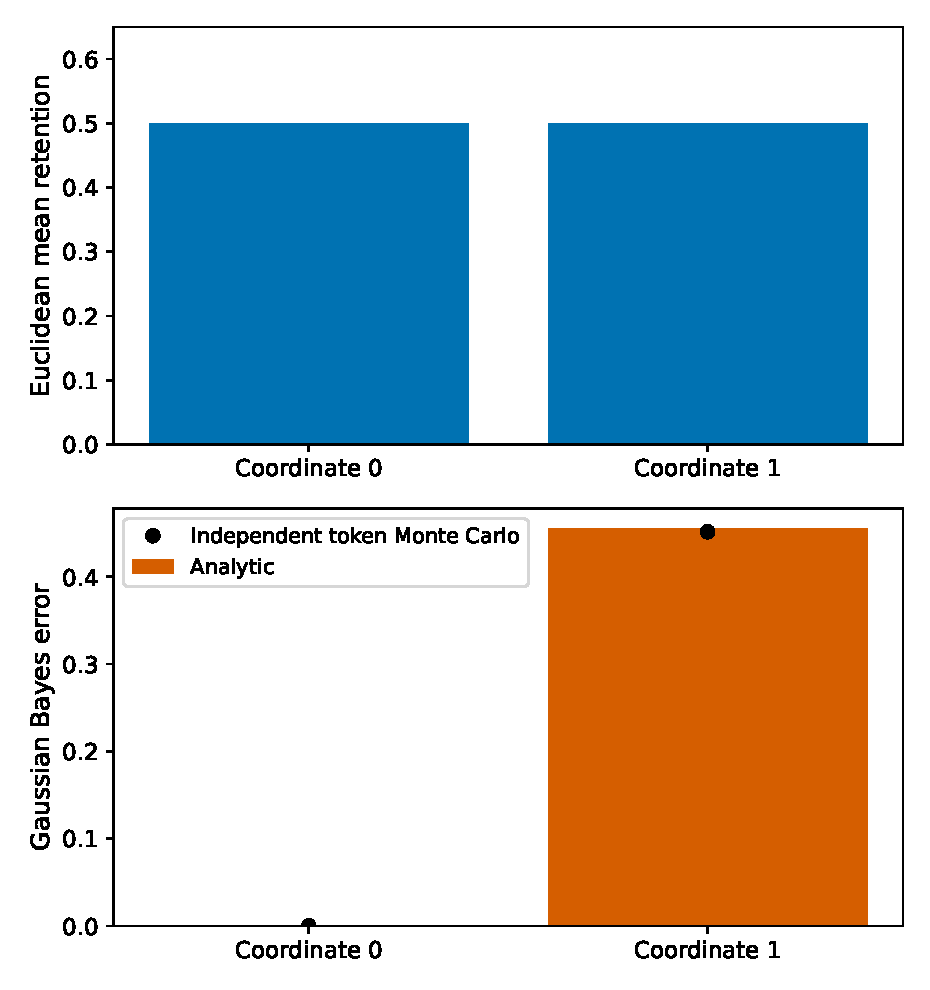
\includegraphics[width=.83\linewidth]{anisotropic_counterexample.pdf}
\caption{Supporting anisotropic Gaussian example: equal retained Euclidean energy need not imply equal optimal risk.}\end{figure}

\section{Preliminary study and detected leakage}
The historical study used seeds 0--4, two CIFAR domains and 2,000 test images per seed. Its initial five-penalty grid and eleven-step LogME were specified before that study. Subsequently, 264/280 validation paths improved from penalty 100 to 1,000, and \LogmeNonconverged{} classwise evidence fits missed their stated convergence criterion. Expanded penalties, adaptive H-score and profile evidence were exploratory corrections. They motivated the unified revision; they do not constitute independently predeclared successes.
The original validation paths improve from penalty 100 to 1,000 in 264 of 280 cases, motivating a separate expanded-grid follow-up rather than a robustness claim from the initial grid. Operators, scores and score-based choices remain fixed; penalties are chosen using validation data only before new test outcomes. The expanded grid reaches $10^8$. 2 of 280 heads select that upper value, while 37 have identical validation accuracy over the largest three penalties; a finite grid still does not prove global optimality. Table~\ref{tab:grid} reports both outcome definitions, so any changed ordering remains visible. The additional diagnostic-probe grid jointly selects candidate and penalty from the same diagnostic label budget; it does not use official-test labels. The lowest observed expanded-grid regret remains covariance retention (0.395 points), closely followed by the fixed-penalty diagnostic probe (0.427). The paired conditional bootstrap interval for their regret difference includes zero; we do not assert statistical superiority. Profile-evidence LogME also improves to 0.4225 points of regret, compared with 0.9225 under the original heads. This stronger evidence baseline further narrows the observed difference from covariance retention. A hindsight audit of all fixed candidates gives p04 dct a mean expanded-grid regret of 0.425 points; this is still not a prospectively chosen rule.

Matching patch size as well as feature budget changes the comparison: expanded-grid within-patch-bank regrets average 0.183 for LogME, 0.211 for covariance retention, and 0.646 for mean retention. These smaller banks have their own oracles and cannot be compared numerically with global-bank regret as though they were the same task. The change in ordering further limits any universal winner claim.

In the diagnostic-label shuffle control, mean retention selects the same candidate in 100\% of the 100 unit/permutation cases. Under the original heads, shuffled-label covariance retention has 0.82 points of mean regret, with its candidate choice changing in all cases. This is a bank-specific negative control: it does not imply that the mean-retention formula is label-independent in general or constitute a formal permutation significance test.
\begin{table}[t]
\centering\small
\caption{Post-primary validation-grid sensitivity (accuracy percentage points). Scores and operator maps are fixed; only downstream penalties are reselected on validation data. Regret uses each head grid's own empirical bank oracle. Diagnostic probe grid, adaptive H-score and profile LogME are exploratory additions.}\label{tab:grid}
\begin{tabular}{lrr}\toprule Selector & Original-grid regret & Expanded-grid regret\\\midrule
Covariance retention & 0.3375 & 0.3950\\
LogME (profile; exploratory) & 0.9225 & 0.4225\\
Diagnostic probe (fixed penalty) & 0.4662 & 0.4275\\
Cross-fitted retention & 0.4750 & 0.5125\\
LogME (11 steps) & 1.0075 & 0.5900\\
Diagnostic probe (grid; exploratory) & 0.6219 & 0.7044\\
Reconstruction energy & 0.7875 & 0.7425\\
Mean retention & 0.7875 & 0.7425\\
H-score (adaptive; exploratory) & 1.5000 & 1.1675\\
Rank (uniform ties) & 2.6591 & 2.4595\\
H-score (fixed shrinkage) & 3.8850 & 2.9875\\
\bottomrule\end{tabular}\end{table}

The historical content audit also identified one operator/diagnostic duplicate at CIFAR-100 seed 1 and one diagnostic/test duplicate at seed 4. An exclusion-only audit holds historical choices and heads fixed and removes the latter test image. Its maximum absolute selected-accuracy change across units/selectors is \RevHistoricalMaxDelta{} percentage points; the pooled covariance-retention regret changes by \RevHistoricalCovDelta{} points. These exact numerical deltas are distributed as CSV. Excluding one test image cannot repair fitting contamination; the final study instead removes content overlap before fitting every operator and head. Differences between historical and final results must not be attributed solely to deduplication, because seeds, test sizes, penalties and baselines also change.

\section{Pretrained rank and optimization controls}
Observed DeiT-tiny and ViT-B/16 patch matrices have different rank properties: the former compresses its 768-dimensional RGB patch space; the latter has full column rank at the observed numerical tolerance. This limits claims that all conventional ViT patch maps necessarily discard dimensions. Conditioning still affects numerical reconstruction and finite-sample regularization.

The historical matched-noise relational control uses identical data, initialization and optimizer with epoch caps 6 and 80, validation-only checkpoint selection and five seeds. The longer-budget tiny ViT solves held-out XOR in all five seeds, reversing the earlier short-budget failure. A raw MLP is a capacity control; CNN outcomes remain variable. A training failure therefore cannot serve as an information-impossibility certificate. These controls support scope restrictions, not the main representation-selection result.
\begin{center}\begin{minipage}{.88\linewidth}\centering
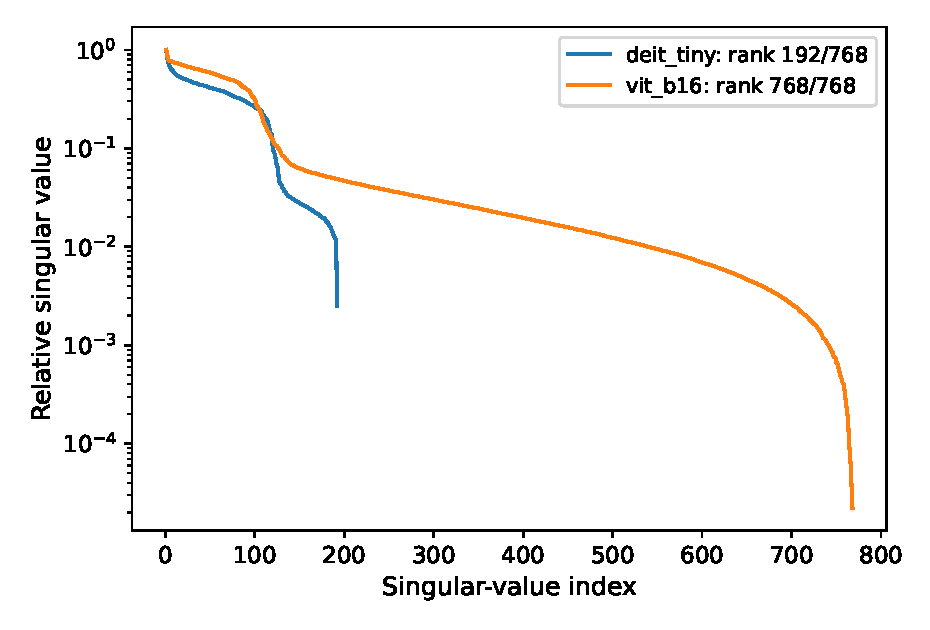
\includegraphics[width=\linewidth]{pretrained_spectra.pdf}
\captionof{figure}{Actual downloaded patch-matrix singular spectra, displayed at readable size. The selection bank transfers only DeiT's patch matrix.}
\end{minipage}\end{center}
\begin{center}\begin{minipage}{.88\linewidth}\centering
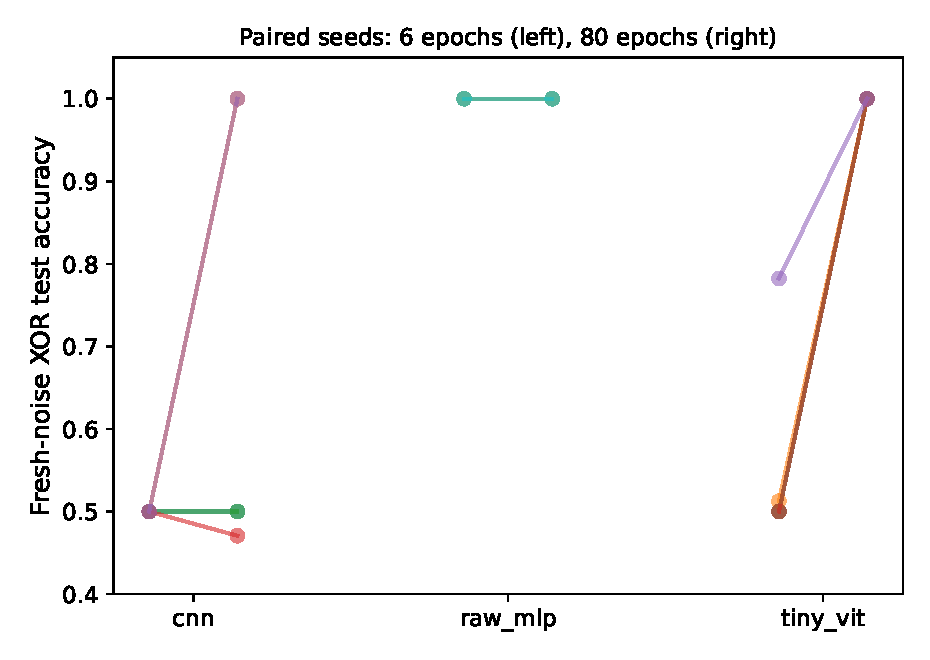
\includegraphics[width=\linewidth]{xor_training_budget.pdf}
\captionof{figure}{Supporting training-budget control, enlarged from the previous combined panel. Every observed seed is retained.}
\end{minipage}\end{center}

\section{Executable reproduction and resource boundary}
The repository's \href{https://github.com/AnkitGuin/Task-Dependent-VIT-Patch-Loss/blob/main/docs/selection_revision_reproducibility.md}{revision reproduction guide} provides the complete command sequence. Its executable entry points are:
\begin{description}
\item[Configuration:] \path{configs/selection_revision.yaml}.
\item[Main execution:] \path{scripts/run_selection_revision.py}.
\item[Independent replay:] \path{scripts/verify_selection_revision.py}.
\item[Isolated resources:] \path{scripts/benchmark_selection_revision.py}.
\item[Tables and figures:] \path{scripts/analyze_selection_revision.py}.
\end{description}
Measurements use a \RevHardware{} CPU with approximately 16 GB RAM, Windows 11 and two numerical-library threads. Cohort manifests record source hashes, dependency versions, hardware and all artifact checksums. Warm/cold selection timings cover the declared selection stage only; downloading, data decoding, imports, selected-head training and final testing are not hidden speedup claims.
\clearpage
\bibliographystyle{plainnat}
\bibliography{references}
\end{document}
